\documentclass[paperwidth=36in,paperheight=48in,portrait,fontscale=0.36]{baposter}
% NIPS Workshops format

% Encoding.
\usepackage[utf8]{inputenc}
\renewcommand{\familydefault}{\sfdefault}
\usepackage{graphicx} % Required for including images
\usepackage{booktabs} % for professional tables
\usepackage{floatrow}
\usepackage{amsmath} % For typesetting math
\usepackage[labelfont=bf, justification=centering]{caption} % Required for specifying captions to tables and figures

\usepackage{multicol} % Required for multiple columns
\setlength{\columnsep}{1cm}
\setlength{\columnseprule}{0.5pt}
\usepackage{multirow}
\usepackage{graphicx}

% For gap between cmidrules.
\usepackage{array}
\newcolumntype{C}{@{\extracolsep{0.1cm}}c@{\extracolsep{0pt}}}%

\newcommand{\compresslist}{ % Define a command to reduce spacing within itemize/enumerate environments, this is used right after \begin{itemize} or \begin{enumerate}
\setlength{\itemsep}{1pt}
\setlength{\parskip}{0pt}
\setlength{\parsep}{0pt}
}

% Defines the color used for content box headers
\definecolor{lightblue}{cmyk}{0.83,0.24,0,0.16}

%%%%%%%%%%%%%%%%%%%%%%%%%%%%%%%%%%%%%%
% macros for the equations
\newcommand{\cw}{\mathbf{cw}}
\newcommand{\cc}{\mathbf{c}}
\newcommand{\kb}{\mathbf{k}}
\newcommand{\mem}{\mathbf{m}}
\newcommand{\rr}{\mathbf{r}}
%%%%%%%%%%%%%%%%%%%%%%%%%%%%%%%%%%%%%%

%%%%%%%%%%%%%%%%%%%%%%%%%%%%%%%%%%%%%%%%%%%%%%%%%%%%%%%%%%%%%%%%%%%%%%%%%%%%%%
%%% Begin of Document
%%%%%%%%%%%%%%%%%%%%%%%%%%%%%%%%%%%%%%%%%%%%%%%%%%%%%%%%%%%%%%%%%%%%%%%%%%%%%%
\frenchspacing

\begin{document}

\hyphenation{resolution occlusions}
%%
\begin{poster}%
  % Poster Options
  {
  % Show grid to help with alignment
  grid=false,
  % Column spacing
  colspacing=1em,
  % Color style
  bgColorOne=white,
  bgColorTwo=white,
  borderColor=lightblue,
  headerColorOne=black,
  headerColorTwo=lightblue,
  headerFontColor=white,
  boxColorOne=white,
  boxColorTwo=lightblue,
  % Format of textbox
  textborder=roundedleft,
%  textborder=faded,
  % Format of text header
  eyecatcher=true,
  headerborder=closed,
  columns=2,
  headerheight=3cm,
%  textfont=\sc, An example of changing the text font
  headershape=roundedright,
  headershade=shadelr,
  headerfont=\Large\bf\textsc, %Sans Serif
  textfont={\setlength{\parindent}{1.5em}\large},
  boxshade=plain,
%  background=shade-tb,
  background=plain,
  linewidth=1pt
  } 
  { % Left Eye Catcher - IBM logo
	
\includegraphics[width=4cm]{../img/ibm_research.png}
  } 
  % Title
  	{\bf\textsc{ On Transfer Learning using a MAC model variant}\vspace{0.2em}}
  % Authors
  {
	\textbf{\null\hfill Vincent Marois \hfill T.S. Jayram \hfill Vincent Albouy \hfill Tomasz Kornuta \hfill\null}\\
	\textbf{\null\hfill Younes Bouhadjar \hfill Ahmet S. Ozcan \hfill\null}\\
	\texttt{\{vmarois,jayram,tkornut,byounes,asozcan\}@us.ibm.com, \{vincent.albouy\}@ibm.com}
  }
  { % Left Eye Catcher
  	
\includegraphics[width=4cm]{../img/arc_logo.png}
  }

%%%%%%%%%%%%%%%%%%%%%%%%%%%%%%%%%%%%%%%%%%%%%%%%%%%%%%%%%%%%%%%%%%%%%%%%%%%%%%%
\headerbox{Contributions}{name=contributions,column=0,row=0}{
\begin{itemize}
	\compresslist
	\item We introduce a \emph{\textbf{simplified}} variant of the MAC (Memory,  Attention,
	and Composition) model~\cite{hudson2018compositional}, which achieves comparable accuracy while training \emph{\textbf{faster}}.
	\item We evaluate both the original MAC model and the simplified variant on CLEVR \& CoGenT datasets, and show that \emph{\textbf{transfer learning with fine-tuning}} results in a \emph{\textbf{15 point increase}} in accuracy, matching the state of the art.
	\item We also demonstrate that \emph{\textbf{improper}} fine-tuning can \emph{\textbf{reduce a model's accuracy}}.
	
\end{itemize}

} %headerbox

\headerbox{The MAC model~\cite{hudson2018compositional}}{name=mac-model, column=0, below=contributions}{
\textbf{MAC network}: a recurrent neural network performing sequential reasoning. At each step, it analyzes the question and shifts the attention over the image.
	\vspace{-3pt}
	\begin{figure}[H]
		\centering
		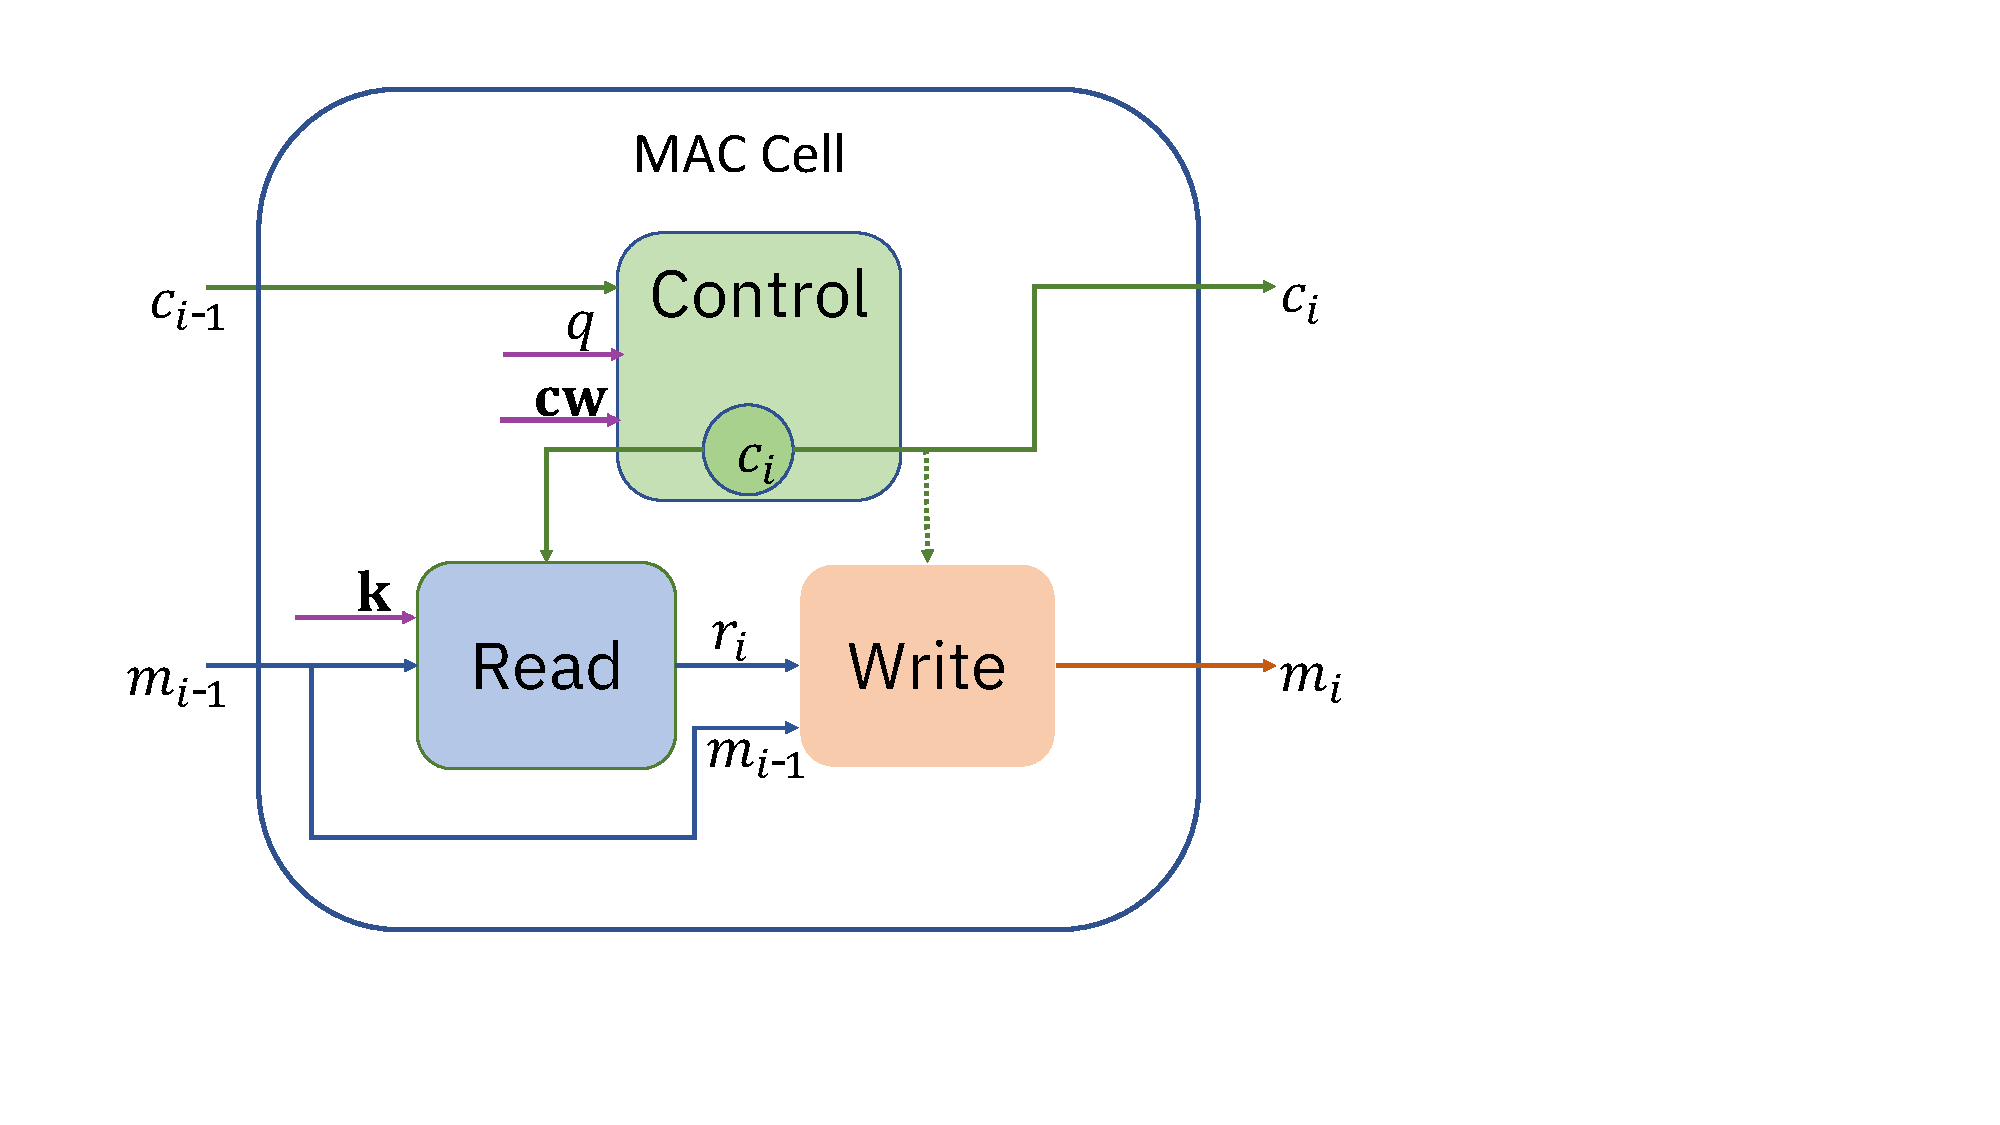
\includegraphics[width=0.4\textwidth]{../img/mac_cell.pdf}
		\caption{\textbf{MAC cell} consists of a control unit, a read unit \& a write unit.}
		\label{fig:mac_cell}
	\end{figure}
	\vspace{-20pt}		 
	\begin{itemize}
	\compresslist
		\item \textbf{Control unit} updates the control state $c_i$ \& shifts the attention over question words.
		\item \textbf{Read unit}, guided by $c_i$, extracts information from the image.
		\item \textbf{Write unit} uses this information to update the memory state $m_i$.
	\end{itemize}
}

\headerbox{The Simplified MAC model (S-MAC)}{name=s-mac, column=0, below=mac-model}{
	
The simplifications are based on two heuristics:
	
\begin{itemize}
		\compresslist
	    \item Taking the MAC cell equations as a whole, all consecutive linear layers (with no non-linear activation in-between) can be combined into a single linear layer.
		\item We assume that dimension-preserving linear layers are invertible so as to avoid information loss.
		\item[$\Rightarrow$] This allows, with a careful reorganization, to apply a single linear layer to the \textit{knowledge base} (feature map extracted from the image) prior to all the reasoning steps and work with this projection throughout the reasoning steps.
\end{itemize}
	

\makebox[\textwidth]{\textbf{MAC \\[5cm] S-MAC}}\\
\vspace{-5pt}
\hrule
\vspace{10pt}
\noindent\textbf{Control unit:} The question $q$ is first made \emph{position-aware} in each reasoning step using an $i$-dependent projection: $q_i = U_i^{[d \times 2d]} q + b_i^{[d]}$.


\begin{multicols}{2}
	\noindent
	\begin{align*}
		&cq_i = W_{cq}^{[d \times 2d]} [c_{i-1}, q_i] + b_{cq}^{[d]}  \tag{c1} \\
		&ca_{is} = W_{ca}^{[1 \times d]} (cq_i \odot \cw_s) + b_{ca}^{[1]}
		\tag{c2.1}\\
		&cv_{is} = \textrm{softmax}(ca_{is}) \tag{c2.2}\\
		&\cc_i = \sum_s cv_{is} \, \cw_s  \tag{c2.3}
	\end{align*}
	\columnbreak
	{\begin{align*}
		&cq_i = W_{cq}^{[d \times d]} c_{i-1} + q_i  \tag{c1} \\
		&ca_{is} = W_{ca}^{[1 \times d]} (cq_i \odot \cw_s)  \tag{c2.1}\\
		&cv_{is} = \textrm{softmax}(ca_{is}) \tag{c2.2}\\
		&\cc_i = \sum_s cv_{is} \, \cw_s  \tag{c2.3}
	\end{align*}}
\end{multicols}

\vskip -0.6cm

\noindent\textbf{Read and write units:}
\begin{multicols}{2}
	\noindent
	\begin{align*}
		&I_{ihw} = (W_{m}^{[d \times d]} \mem_{i-1} + b_{m}^{[d]}) \\
		& \qquad \quad \odot (W_{k}^{[d \times d]} \kb_{hw} + b_{k}^{[d]}) \tag{r1} \\
		&I'_{ihw} =  W_{I'}^{[d \times 2d]} [I_{ihw},\kb_{hw}]  + b_{I'}^{[d]}  \tag{r2} \\
		&ra_{ihw} = W_{ra}^{[1 \times d]} (\cc_i \odot I'_{ihw}) + b_{ra}^{[1]} \tag{r3.1}\\
		&rv_{ihw} = \textrm{softmax}(ra_{ihw}) \tag{r3.2}\\
		&\rr_i = \sum_s rv_{ihw} \, \kb_{hw}  \tag{r3.3}\\
		&\mem_i = W_{rm}^{[d \times 2d]} [\rr_i, \mem_{i-1}]  + b_{rm}^{[d]} \tag{w1}
	\end{align*}
	\columnbreak
	{\begin{align*}
		&\\
		&I_{ihw} = \mem_{i-1} \odot \kb_{hw} \tag{r1} \\ 
		&I'_{ihw} = W_{I'}^{[d \times d]} I_{ihw} + b_{I'}^{[d]} + \kb_{hw} \tag{r2} \\
		&ra_{ihw} = W_{ra}^{[1 \times d]} (\cc_i \odot I'_{ihw})  \tag{r3.1}\\
		&rv_{ihw} = \textrm{softmax}(ra_{ihw}) \tag{r3.2}\\
		&\rr_i = \sum_s rv_{ihw} \, \kb_{hw}  \tag{r3.3}\\
		&\mem_i = W_{rm}^{[d \times d]} \rr_i + b_{rm}^{[d]} \tag{w1}
	\end{align*}}
\end{multicols}

\vspace{-15pt}
\begin{table}[H]
	\centering
	\caption{Comparison of numbers of position-independent parameters between MAC \& S-MAC cells.}
	\begin{tabular}{llll}
		\toprule
		Model        & Read Unit               & Write Unit &  Control Unit         \\
		\midrule
		MAC   &  787,969 &  524,800        &    525,313    \\
		S-MAC & 263,168  & 262,656       &    263,168 \\
		\midrule
		Reduction by [\%]  & 67\%  &   50\%       &      50\%  \\
		\bottomrule
	\end{tabular}
	\label{tab:mac_cell_parameters}
\end{table}

}

\headerbox{Links}{name=links,column=0,below=s-mac}{
	\vspace{-15pt}
	\null\hfill
	\begin{minipage}[H]{0.3\textwidth}
		\begin{figure}[H]
			
\includegraphics[width=0.6\textwidth]{../img/reproducible_research_qr_code.png}
			\vspace{-15pt}
			\caption*{\textbf{How to reproduce the experiments.}}
			\label{fig:qr_repro_research}
		\end{figure}
	\end{minipage}
	\hfill
	\begin{minipage}[H]{0.3\textwidth}
		\begin{figure}[H]
			
\includegraphics[width=0.7\textwidth]{../img/arxiv_paper_qr_code.png}
			\vspace{-15pt}
			\caption*{Paper on arXiv.}
			\label{fig:qr_arxiv}
		\end{figure}
	\end{minipage}
	\hfill
	\begin{minipage}[H]{0.3\textwidth}
		\begin{figure}[H]
			
\includegraphics[width=0.7\textwidth]{../img/clevr_qr_code.png}
			\vspace{-15pt}
			\caption*{CLEVR Dataset.}
			\label{fig:qr_clevr}
		\end{figure}
	\end{minipage}
	\hfill\null
}

\headerbox{The CLEVR \& CoGenT datasets}{name=datasets, column=1}{
	\vspace{-10pt}
	\begin{figure}[H]
		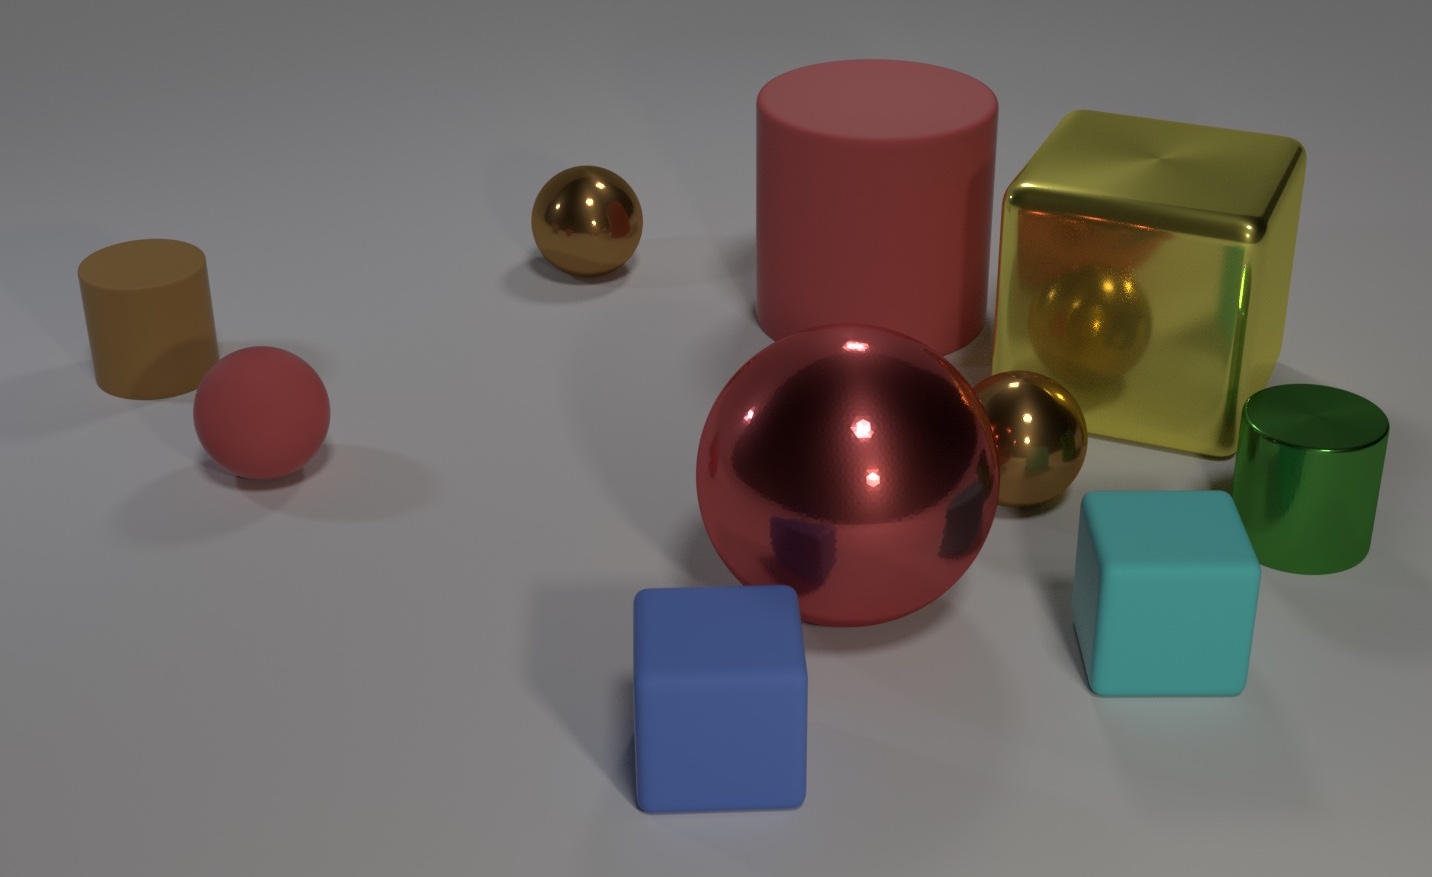
\includegraphics[width=0.4\textwidth]{../img/teaser.jpg}
		\caption{\textbf{Q}: \textit{How many objects are either small cylinders or red things?} \textbf{A}: 5.}
		\label{fig:clevr_task}
	\end{figure}
	\vspace{-20pt}
	\begin{itemize}
	  	\compresslist
	  	\item The authors of CLEVR~\cite{johnson2017clevr} also introduced a variant called CLEVR-CoGenT, aiming at evaluation of how well models can learn compositional concepts.
	  	\item Similar to CLEVR, but with two conditions, as follows:
	\end{itemize}
	\vspace{-10pt}
	\begin{table}[H]
		\centering
		\begin{tabular}{llll}
			\toprule
			Dataset        & Cubes              & Cylinders &  Spheres         \\
			\midrule
			CLEVR   &  any color &  any color        &    any color    \\
			CLEVR CoGenT-A & gray / blue / brown / yellow  & red / green / purple / cyan       &    any color  \\
			CLEVR CoGenT-B  & red / green / purple / cyan &   gray / blue / brown / yellow       &      any color  \\
			\bottomrule
		\end{tabular}
		\caption{Colors/shapes combinations present in CLEVR, CoGenT-A and CoGenT-B datasets.}
		\label{tab:cogent_conditions}
	\end{table}
	
}

\headerbox{Experiments \& results}{name=experiments, column=1, below=datasets}{
	\vspace{-10pt}
	\begin{table}[H]
	\centering
	\scalebox{1}{
	\begin{tabular}{cccccccc}
		\toprule
		\multirow{2}{*}{Model} & \multicolumn{3}{c}{Training} &  \multicolumn{2}{c}{Fine-tuning} & \multicolumn{2}{c}{Test} \\
		\cmidrule{2-4} \cmidrule{5-6} \cmidrule{7-8} 
		& Dataset                & Time [h:m] & Acc [\%]          & Dataset & Acc [\%]  & Dataset & Acc [\%] \\
		\midrule
		MAC & CLEVR  & 30:52  & 96.70 & --   & --  & CLEVR    & 96.17 \\
		\cmidrule{1-8}
		\cmidrule{1-8}
		
		\multirow{13}{*}{S-MAC} & CLEVR  & 28:30  & 95.82 & --   & --  & CLEVR    & 95.29 \\
		\cmidrule{2-4} \cmidrule{5-6} \cmidrule{7-8} 
		
		& CoGenT-A  & 28:33   & 96.09 &  --  &  --  & CoGenT-A & 95.91 \\
		\cmidrule{2-4} \cmidrule{5-6} \cmidrule{7-8} 
		
		
		& \multirow{2}{*}{CLEVR}  & \multirow{2}{*}{28:30}  & \multirow{2}{*}{95.82} & \multirow{2}{*}{--}   & \multirow{2}{*}{--}  &   CoGenT-A    &  95.47 \\
		\cmidrule{7-8} 
		&                        &   &              &     &                               & CoGenT-B   &  95.58  \\		
		
		\cmidrule{2-4} \cmidrule{5-6} \cmidrule{7-8} 
		& \multirow{4}{*}{CoGenT-A}   & \multirow{4}{*}{28:33}   & \multirow{4}{*}{96.09}  &  \multirow{1}{*}{--}  &  \multirow{1}{*}{--}   & CogenT-B & 78.71 \\
		\cmidrule{5-6} \cmidrule{7-8} 
		&                             &                                         &    &   \multirow{2}{*}{CoGenT-B}         &       \multirow{2}{*}{96.85}          & CoGenT-A &  91.24 \\
		\cmidrule{7-8} 
		&                             &                                         &       &         &                & CoGenT-B &    94.55 \\
		
		\cmidrule{2-4} \cmidrule{5-6} \cmidrule{7-8} 
		& \multirow{2}{*}{CLEVR}  & \multirow{2}{*}{28:30}  & \multirow{2}{*}{95.82} &   \multirow{2}{*}{CoGenT-B}         &       \multirow{2}{*}{97.67}          & CoGenT-A &  92.11 \\
		\cmidrule{7-8} 
		&                             &                                         &       &         &                & CoGenT-B &    92.95 \\  		
		
		
		\bottomrule
	\end{tabular}}
	\caption{CLEVR \& CoGenT accuracies for the MAC \& S-MAC models.}
	\label{tab:data_properties}
\end{table}
\vspace{-20pt}

\begin{itemize}
	\compresslist
	\item Our experiments on \emph{zero-shot learning} (CoGenT-A $\rightarrow$ CoGenT-B) show that both models have poor performance, in line with
	the other models in the literature.
	\item With fine-tuning, both MAC models match state-of-the-art accuracy (a 15pts increase).
	\item \textbf{S-MAC presents a 10\% speed-up in training time and comparable accuracy.}
	\item Finetuning CLEVR-trained models on CoGenT-A or -B hurts their generalization capabilities.
	\item[$\Rightarrow$] \emph{Zero-shot learning} remains an interesting problem to solve.
\end{itemize}

}

\headerbox{Compositional generalization of the MAC model}{name=mac-failures, column=1, below=experiments}{
	\vspace{-10pt}
	\begin{figure}[H]
		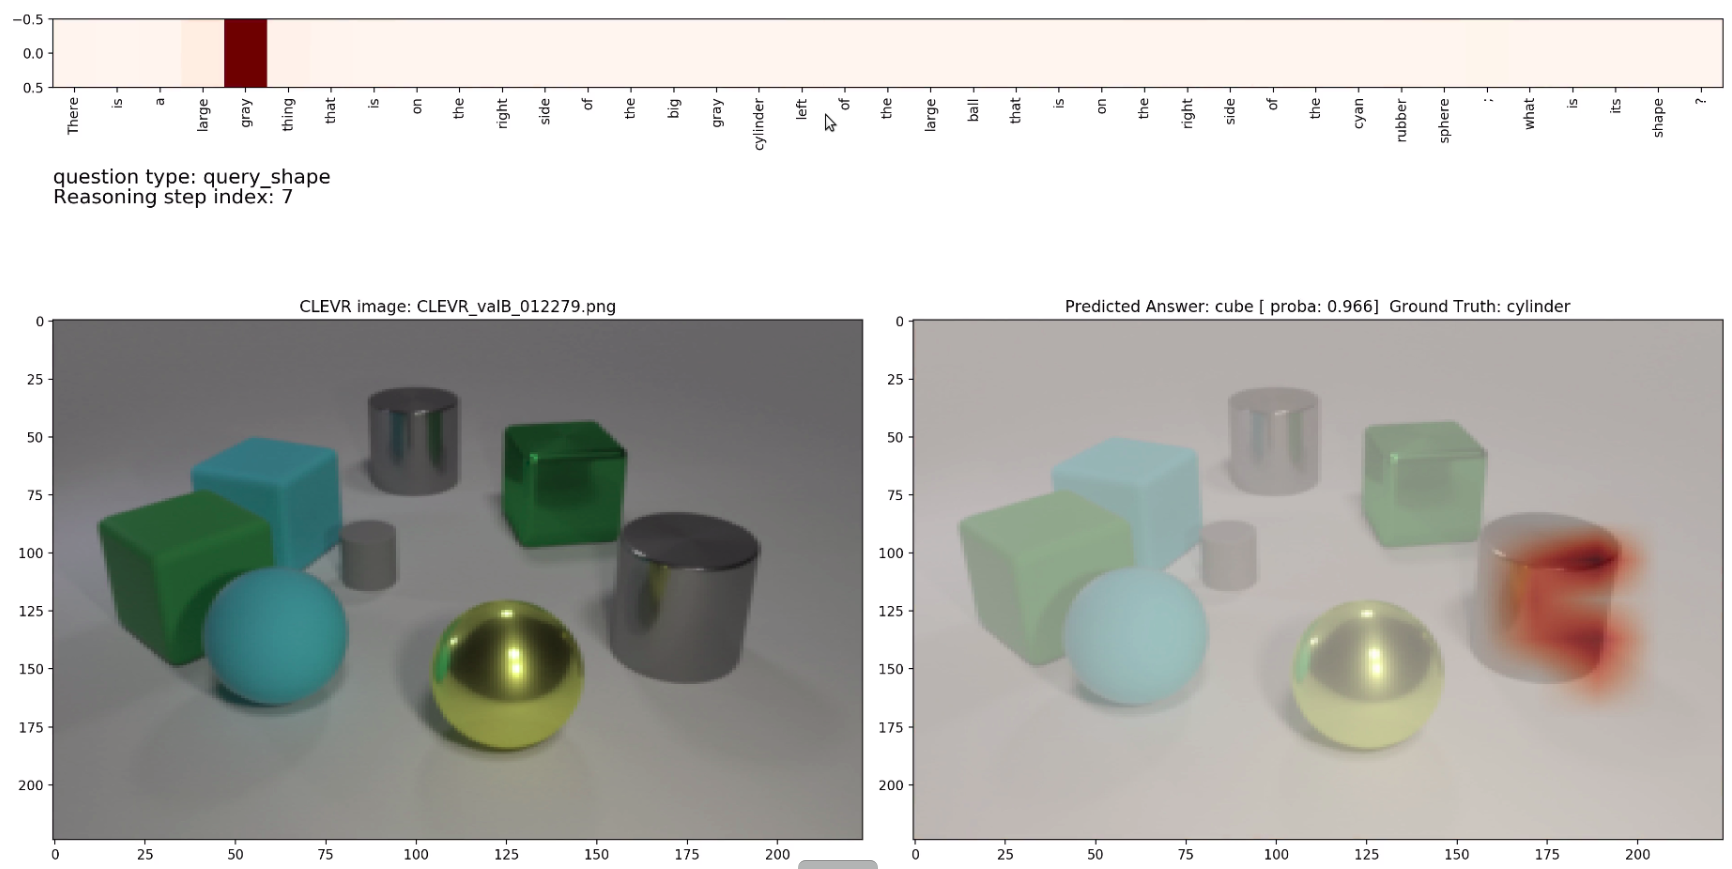
\includegraphics[width=0.71\textwidth]{../img/fail_mac_cogent_b_shape.png}
		\caption{There is a large gray thing that is on the right side of the big gray cylinder left of the large ball that is on the right side if the cyan rubber sphere; what is its shape?}
		\label{fig:mac_failure}
	\end{figure}
	\vspace{-20pt}
	\begin{itemize}
		\compresslist
		\item Asked about the shape of the leftmost \textbf{gray cylinder}, the model correctly finds it, (cf. \emph{visual attention map}), and refers to it using its color (\emph{attention over the question words}).
		\item As it never saw \textbf{gray cylinders} during training, whereas learned the \textbf{gray cubes} compositional concept, the model predicts the shape as a \textbf{cube}.
		\item[$\Rightarrow$] This indicates that MAC does not separate shape from color, but has a better understanding of color cues (as it found the object by its color).
	\end{itemize}
}

\headerbox{References}{name=references, column=1, below=mac-failures}{
	\small
	\vspace{-8pt}
	\renewcommand{\refname}{}
	\bibliographystyle{alpha}
	\bibliography{../vigil_bibliography}
}

\end{poster}
\end{document}